\documentclass{beamer}
\usepackage{xcolor}
\usepackage{relsize}

\newcommand{\nfour}{${\cal N}=4\;$}
\newcommand{\ntwo}{${\mathcal N}=2\;$}
\newcommand{\none}{${\mathcal N}=1\,$}
\newcommand{\ntt}{${\mathcal N}=(2,2)\,$}
\newcommand{\nzt}{${\mathcal N}=(0,2)\,$}
\newcommand{\cpn}{CP$^{(N-1)}\,$}
\newcommand{\ca}{{\mathcal A}}
\newcommand{\cell}{{\mathcal L}}
\newcommand{\cw}{{\mathcal W}}
\newcommand{\cs}{{\mathcal S}}
\newcommand{\vp}{\varphi}
\newcommand{\pt}{\partial}
\newcommand{\ve}{\varepsilon}
\newcommand{\gs}{g^{2}}
\newcommand{\zn}{$Z_N$}
\newcommand{\cd}{${\mathcal D}$}
\newcommand{\cde}{{\mathcal D}}
\newcommand{\cf}{${\mathcal F}$}
\newcommand{\cfe}{{\mathcal F}}

\newcommand{\gsim}{\lower.7ex\hbox{$
\;\stackrel{\textstyle>}{\sim}\;$}}
\newcommand{\lsim}{\lower.7ex\hbox{$
\;\stackrel{\textstyle<}{\sim}\;$}}

\renewcommand{\theequation}{\thesection.\arabic{equation}}

%%%%%%%%%%%%%
%%%%%%%%%%%
%% common definitions
\def\stackunder#1#2{\mathrel{\mathop{#2}\limits_{#1}}}
\def\beqn{\begin{eqnarray}}
\def\eeqn{\end{eqnarray}}
\def\nn{\nonumber}
\def\baselinestretch{1.1}
\def\beq{\begin{equation}}
\def\eeq{\end{equation}}
\def\ba{\beq\new\begin{array}{c}}
\def\ea{\end{array}\eeq}
\def\be{\ba}
\def\ee{\ea}
\def\stackreb#1#2{\mathrel{\mathop{#2}\limits_{#1}}}
\def\Tr{{\rm Tr}}
%\newcommand{\gsim}{\lower.7ex\hbox{$\;\stackrel{\textstyle>}{\sim}\;$}}
% \newcommand{\lsim}{\lower.7ex\hbox{$
%\;\stackrel{\textstyle<}{\sim}\;$}}
%\newcommand{\nfour}{${\mathcal N}=4$ }
%\newcommand{\ntwo}{${\mathcal N}=2$ }
\newcommand{\ntwon}{${\mathcal N}=2$}
\newcommand{\ntwot}{${\mathcal N}= \left(2,2\right) $ }
\newcommand{\ntwoo}{${\mathcal N}= \left(0,2\right) $ }
%\newcommand{\none}{${\mathcal N}=1$ }
\newcommand{\nonen}{${\mathcal N}=1$}
%\newcommand{\vp}{\varphi}
%\newcommand{\pt}{\partial}
%\newcommand{\ve}{\varepsilon}
%\newcommand{\gs}{g^{2}}
%\newcommand{\qt}{\tilde q}
\renewcommand{\theequation}{\thesection.\arabic{equation}}

%%
\newcommand{\p}{\partial}
\newcommand{\wt}{\widetilde}
\newcommand{\ov}{\overline}
\newcommand{\mc}[1]{\mathcal{#1}}
\newcommand{\md}{\mathcal{D}}

\newcommand{\GeV}{{\rm GeV}}
\newcommand{\eV}{{\rm eV}}
\newcommand{\Heff}{{\mathcal{H}_{\rm eff}}}
\newcommand{\Leff}{{\mathcal{L}_{\rm eff}}}
\newcommand{\el}{{\rm EM}}
\newcommand{\uflavor}{\mathbf{1}_{\rm flavor}}
\newcommand{\lgr}{\left\lgroup}
\newcommand{\rgr}{\right\rgroup}

\newcommand{\Mpl}{M_{\rm Pl}}
\newcommand{\suc}{{{\rm SU}_{\rm C}(3)}}
\newcommand{\sul}{{{\rm SU}_{\rm L}(2)}}
\newcommand{\sutw}{{\rm SU}(2)}
\newcommand{\suth}{{\rm SU}(3)}
\newcommand{\ue}{{\rm U}(1)}
%%%%%%%%%%%%%%%%%%%%%%%%%%%%%%%%%%%%%%%
%  Slash character...
\def\slashed#1{\setbox0=\hbox{$#1$}             % set a box for #1
   \dimen0=\wd0                                 % and get its size
   \setbox1=\hbox{/} \dimen1=\wd1               % get size of /
   \ifdim\dimen0>\dimen1                        % #1 is bigger
      \rlap{\hbox to \dimen0{\hfil/\hfil}}      % so center / in box
      #1                                        % and print #1
   \else                                        % / is bigger
      \rlap{\hbox to \dimen1{\hfil$#1$\hfil}}   % so center #1
      /                                         % and print /
   \fi}                                        %

%%EXAMPLE:  $\slashed{E}$ or $\slashed{E}_{t}$

%%

\newcommand{\LN}{\Lambda_\text{SU($N$)}}
\newcommand{\sunu}{{\rm SU($N$) $\times$ U(1) }}
\newcommand{\sunun}{{\rm SU($N$) $\times$ U(1)}}
\def\cfl {$\text{SU($N$)}_{\rm C+F}$ }
\def\cfln {$\text{SU($N$)}_{\rm C+F}$}
\newcommand{\mUp}{m_{\rm U(1)}^{+}}
\newcommand{\mUm}{m_{\rm U(1)}^{-}}
\newcommand{\mNp}{m_\text{SU($N$)}^{+}}
\newcommand{\mNm}{m_\text{SU($N$)}^{-}}
\newcommand{\AU}{\mc{A}^{\rm U(1)}}
\newcommand{\AN}{\mc{A}^\text{SU($N$)}}
\newcommand{\aU}{a^{\rm U(1)}}
\newcommand{\aN}{a^\text{SU($N$)}}
\newcommand{\baU}{\ov{a}{}^{\rm U(1)}}
\newcommand{\baN}{\ov{a}{}^\text{SU($N$)}}
\newcommand{\lU}{\lambda^{\rm U(1)}}
\newcommand{\lN}{\lambda^\text{SU($N$)}}
%\newcommand{\Tr}{{\rm Tr\,}}
\newcommand{\bxir}{\ov{\xi}{}_R}
\newcommand{\bxil}{\ov{\xi}{}_L}
\newcommand{\xir}{\xi_R}
\newcommand{\xil}{\xi_L}
\newcommand{\bzl}{\ov{\zeta}{}_L}
\newcommand{\bzr}{\ov{\zeta}{}_R}
\newcommand{\zr}{\zeta_R}
\newcommand{\zl}{\zeta_L}
\newcommand{\nbar}{\ov{n}}

\newcommand{\CPC}{CP$^{N-1}$)$\times$C }
\newcommand{\CPCn}{CP$^{N-1}$)$\times$C}

\newcommand{\lar}{\lambda_R}
\newcommand{\lal}{\lambda_L}
\newcommand{\larl}{\lambda_{R,L}}
\newcommand{\lalr}{\lambda_{L,R}}
\newcommand{\bla}{\ov{\lambda}}
\newcommand{\blar}{\ov{\lambda}{}_R}
\newcommand{\blal}{\ov{\lambda}{}_L}
\newcommand{\blarl}{\ov{\lambda}{}_{R,L}}
\newcommand{\blalr}{\ov{\lambda}{}_{L,R}}

\newcommand{\bgamma}{\ov{\gamma}}
\newcommand{\bpsi}{\ov{\psi}{}}
\newcommand{\bphi}{\ov{\phi}{}}
\newcommand{\bxi}{\ov{\xi}{}}


\newcommand{\hphi}{\hat\phi{}}
\newcommand{\hbphi}{\hat{\ov\phi}{}}
\newcommand{\hxi}{\hat\xi{}}
\newcommand{\hbxi}{\hat{\ov\xi}{}}
\newcommand{\hsigma}{\hat\sigma{}}
\newcommand{\hbsigma}{\hat{\ov\sigma}{}}
\newcommand{\hlambda}{\hat\lambda{}}
\newcommand{\hblambda}{\hat{\ov\lambda}{}}
\newcommand{\hz}{\hat z{}}
\newcommand{\hbz}{\hat{\ov z}{}}
\newcommand{\hzeta}{\hat\zeta{}}
\newcommand{\hbzeta}{\hat{\ov\zeta}{}}


\newcommand{\ff}{\mc{F}}
\newcommand{\bff}{\ov{\mc{F}}}

\newcommand{\eer}{\epsilon_R}
\newcommand{\eel}{\epsilon_L}
\newcommand{\eerl}{\epsilon_{R,L}}
\newcommand{\eelr}{\epsilon_{L,R}}
\newcommand{\beer}{\ov{\epsilon}{}_R}
\newcommand{\beel}{\ov{\epsilon}{}_L}
\newcommand{\beerl}{\ov{\epsilon}{}_{R,L}}
\newcommand{\beelr}{\ov{\epsilon}{}_{L,R}}

\newcommand{\bi}{{\bar \imath}}
\newcommand{\bj}{{\bar \jmath}}
\newcommand{\bk}{{\bar k}}
\newcommand{\bl}{{\bar l}}
\newcommand{\bmm}{{\bar m}}
\newcommand{\bp}{{\bar p}}
\newcommand{\bkk}{{\bar k}}
\newcommand{\br}{{\bar r}}

\newcommand{\nz}{{n^{(0)}}}
\newcommand{\no}{{n^{(1)}}}
\newcommand{\bnz}{{\ov{n}{}^{(0)}}}
\newcommand{\bno}{{\ov{n}{}^{(1)}}}
\newcommand{\Dz}{{D^{(0)}}}
\newcommand{\Do}{{D^{(1)}}}
\newcommand{\bDz}{{\ov{D}{}^{(0)}}}
\newcommand{\bDo}{{\ov{D}{}^{(1)}}}
\newcommand{\sigz}{{\sigma^{(0)}}}
\newcommand{\sigo}{{\sigma^{(1)}}}
\newcommand{\bsigz}{{\ov{\sigma}{}^{(0)}}}
\newcommand{\bsigo}{{\ov{\sigma}{}^{(1)}}}

\newcommand{\rrenz}{{r_\text{ren}^{(0)}}}
\newcommand{\bren}{{\beta_\text{ren}}}

\newcommand{\mbps}{m_{\text{\tiny BPS}}}
\newcommand{\W}{\mathcal{W}}
\newcommand{\M}{\mathcal{M}}
\newcommand{\bM}{\ov{\mathcal{M}}{}}
\newcommand{\Q}{\mathcal{Q}}
\newcommand{\bQ}{\ov{\mathcal{Q}}{}}
\newcommand{\D}{\mathcal{D}}
\newcommand{\V}{\mathcal{V}}

\newcommand{\cp}{$\text{CP}^{N-1}$\,\,}

\usefonttheme{serif}
\usetheme{AnnArbor}

\setbeamertemplate{background canvas}[vertical shading][bottom=yellow!80,top=yellow!30]
\setbeamertemplate{blocks}[rounded][shadow=true]

\setbeamercolor{normal text}{fg=blue!80}
\setbeamercolor{alerted text}{fg=orange!90}
\setbeamercolor{math text}{fg=red!90}

\title[Effective Action of \cp]
      {Low-Energy Effective Action\\
       of \cp Model at large $ N $}

\author{Pavel A. Bolokhov}

\date{May 14, 2016}

\institute[University of Minnesota Duluth \& SPbSU]{University of Minnesota Duluth}

\begin{document}

\maketitle




%%%%%%%%%%%%%%%%%%%%%%%%%%%%%%%%%%%%%%%%%%%%%%%%%%%%%%%%%%%%%%%%%%
%%%%%%%%%%%%%%%%%%%%%%%%%%%%%%%%%%%%%%%%%%%%%%%%%%%%%%%%%%%%%%%%%%
\section{Non-abelian Vortices}
%%%%%%%%%%%%%%%%%%%%%%%%%%%%%%%%%%%%%%%%%%%%%%%%%%%%%%%%%%%%%%%%%%
%%%%%%%%%%%%%%%%%%%%%%%%%%%%%%%%%%%%%%%%%%%%%%%%%%%%%%%%%%%%%%%%%%
\begin{frame}{}
\usefont{T1}{ptm}{m}{n}\fontsize{60pt}{60pt}\selectfont
\begin{center}
        Vortices
\end{center}
\end{frame}


%%%%%%%%%%%%%%%%%%%%%%%%%%%%%%%%%%%%%%%%%%%%%%%%%%%%%%%%%%%%%%%%%%
\begin{frame}{Non-Abelian vortices}

  Non-abelian vortices appear in \ntwo $ U(N) $ SQCD, $ N_c ~=~ N_f $\\
  {\tiny\sc [M.Shifman, A.Yung] [A.Hanany, D.Tong] [N.Dorey]}
  \begin{align*}
    %
    V(q^A,\wt{q}{}_A,a^a,a) &~~=~~
    \frac{g_2^2}{2} \left( \frac{1}{g_2^2}f^{abc}\ov{a}{}^b a^c  ~+~
    \ov{q}{}_A T^a q^A  - \wt{q}{}_A T^a \ov{\wt{q}}{}^A \right)^2 \\
    %
    & ~~+~~ \frac{g_1^2}{8}\, \left(\ov{q}{}_A q^A ~-~ \wt{q}{}_A\ov{\wt{q}}{}^A ~-~ N\,\xi_3 \right)^2 \\
    %
    & ~~+~~ 2\,g_2^2 \left| \wt{q}{}_A T^a q^A \right|^2 ~+~
    \frac{g_1^2}{2} \left| \wt{q}_A q^A ~-~ \frac{N}{2}\, \xi \right|^2 \\
    %
    & ~~+~~ \frac{1}{2} \sum_{A=1}^N \Biggl\{ \left|\left(a ~+~ \sqrt{2}m_A ~+~ 2T^a a^a\right)q^A\right|^2 \\
    %
    & \phantom{\frac{1}{2}\sum_{A=1}^N \Biggl\{ } ~~+~~
    \left| \left( a ~+~ \sqrt{2}m_A ~+~ 2T^a a^a\right) \ov{\wt{q}}^A \right|^2 \Biggr\}~.
    \end{align*}
  
\end{frame}


%%%%%%%%%%%%%%%%%%%%%%%%%%%%%%%%%%%%%%%%%%%%%%%%%%%%%%%%%%%%%%%%%%
\begin{frame}

  The $ Z_N $ string solution
  \begin{center}
    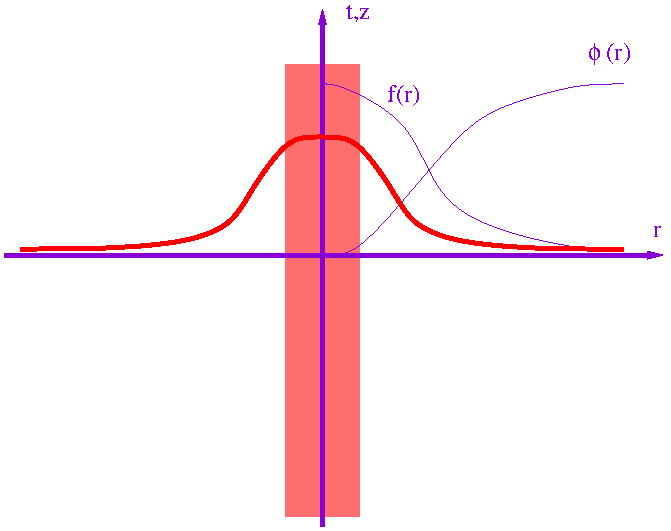
\includegraphics[width=9.0cm,decodearray={0.2 0.5}]{string.pdf}
  \end{center}

\end{frame}


%%%%%%%%%%%%%%%%%%%%%%%%%%%%%%%%%%%%%%%%%%%%%%%%%%%%%%%%%%%%%%%%%%
\begin{frame}
  
The $ Z_N $ string solution
\begin{align*}
  %
  \varphi ~~=~~ & \lgr \begin{matrix}
    \phi_2(r)  & 0  & \ldots & 0 \\
    \ldots  &  \ldots & \ldots & \ldots \\
    0  & \ldots      & \phi_2(r) &  0 \\
    0  & 0           & \ldots  &   e^{i\alpha} \phi_1(r)
  \end{matrix}        \rgr     \\
  %
  A_i^{\rm SU(N)} ~~=~~ \frac{1}{N} & \lgr \begin{matrix}
    1  & \ldots & 0 & 0 \\
    \ldots & \ldots & \ldots & \ldots \\
    0  & \ldots  & 1  &  0 \\
    0  & 0   & \ldots  &  - (N-1)
  \end{matrix} \rgr  \times \\
  %
  &       \qquad\qquad\qquad\qquad     \times(\p_i \alpha) \lgr  -1 ~+~ f_{NA}(r) \rgr  \\
  %
  A_i^{\rm U(1)} ~~=~~ & \frac{1}{N} (\p_i \alpha) \lgr 1 ~-~ f(r) \rgr
  %                       A_0^{\rm U(1)} ~~=~~ A_0^{\rm SU(N)} ~~=~~ 0~.
\end{align*}
\end{frame}


%%%%%%%%%%%%%%%%%%%%%%%%%%%%%%%%%%%%%%%%%%%%%%%%%%%%%%%%%%%%%%%%%%
\begin{frame}
	In the singular gauge, it is the gauge field that winds, now around the origin

\begin{align*}
%
	A_i^{\rm SU(N)} ~~=~~ \frac{1}{N}\, &\, U\, \lgr \begin{matrix}
					          	1  & \ldots & 0 & 0 \\
						  	\ldots & \ldots & \ldots & \ldots \\
							0  & \ldots  & 1  &  0 \\
							0  & 0   & \ldots  &  - (N-1) 
					         \end{matrix} \rgr  \, U^{-1} \times \\
%
			&	\qquad\qquad\qquad\qquad\qquad     \times(\p_i \alpha)\, f_{NA}(r)  \\
%
	A_i^{\rm U(1)} ~~=~~ -\, & \frac{1}{N}\, (\p_i \alpha)\, f(r) 
%			A_0^{\rm U(1)} ~~=~~ A_0^{\rm SU(N)} ~~=~~ 0~.
\end{align*}

	The rotation matrix $U$ provides the {\it orientation} of the string in the $ SU(N) $ space
\end{frame}


%%%%%%%%%%%%%%%%%%%%%%%%%%%%%%%%%%%%%%%%%%%%%%%%%%%%%%%%%%%%%%%%%%
\begin{frame}
\vspace*{\fill}
	The string solution breaks
\[
	\frac{SU(N)}
            {SU(N-1) \times U(1)}         ~~\sim~~  CP(N-1)~\text.
\]
\vspace*{\fill}
\end{frame}


%%%%%%%%%%%%%%%%%%%%%%%%%%%%%%%%%%%%%%%%%%%%%%%%%%%%%%%%%%%%%%%%%%%%%%%%%%%%%%%%%%%%%
%%%%%%%%%%%%%%%%%%%%%%%%%%%%%%%%%%%%%%%%%%%%%%%%%%%%%%%%%%%%%%%%%%%%%%%%%%%%%%%%%%%%%
\begin{frame}
	The string orientation $ U $ can be unambigiously parametrized by the modulus $ n^l \in C $:
\[
	\frac{1}{N}\, U \, \lgr \begin{matrix}
				  1  & \ldots & 0 & 0 \\
				  \ldots & \ldots & \ldots & \ldots \\
				  0 & \ldots & 1 & 0  \\
				  0 & 0 & \ldots & -(N-1) 
				\end{matrix} \rgr
			U^{-1}  
	~~=~~
	-\, n^i\,\ov{n}{}_l  ~~+~~ \frac{1}{N}\cdot{\mathlarger{\mathbf{1}}}{}^i_{~l} 
\]
	with a condition
\[
	\ov{n}{}_l \cdot n^l ~~=~~ 1 \text.
\]
	Thus $ n^l $ are \emph{orientational} collective coordinates

	This defines $ 2(N - 1) $ degrees of freedom, since \cp theory can be obtained from a gauge
	theory, and one phase can be removed

\end{frame}




%%%%%%%%%%%%%%%%%%%%%%%%%%%%%%%%%%%%%%%%%%%%%%%%%%%%%%%%%%%%%%%%%%
%%%%%%%%%%%%%%%%%%%%%%%%%%%%%%%%%%%%%%%%%%%%%%%%%%%%%%%%%%%%%%%%%%
\section{\cp Model}
%%%%%%%%%%%%%%%%%%%%%%%%%%%%%%%%%%%%%%%%%%%%%%%%%%%%%%%%%%%%%%%%%%
%%%%%%%%%%%%%%%%%%%%%%%%%%%%%%%%%%%%%%%%%%%%%%%%%%%%%%%%%%%%%%%%%%
\begin{frame}{}
\usefont{T1}{ptm}{m}{n}\fontsize{60pt}{60pt}\selectfont
\begin{center}
        $\text{CP}^{N-\mathsmaller{1}}$ Model
\end{center}
\end{frame}


%%%%%%%%%%%%%%%%%%%%%%%%%%%%%%%%%%%%%%%%%%%%%%%%%%%%%%%%%%%%%%%%%%
\begin{frame}{Bosonic theory}

	The non-supersymmetric \cp describes a complex vector 
\[
	n^l\,,\qquad\qquad l ~=~ 1\,,\, ...\,,\, N
\]
	subject to the identification
\[
	\vec{n} ~~\sim~~ \lambda\, \vec{n}\,,
	\qquad\qquad \lambda ~\in~ \mathcal{C}
\]


\end{frame}


%%%%%%%%%%%%%%%%%%%%%%%%%%%%%%%%%%%%%%%%%%%%%%%%%%%%%%%%%%%%%%%%%%
\begin{frame}{}

	The {\it gauge} formulation for such a theory was introduced by Witten
\[
 	\mc{L} ~~=~~
		\,\frac{1}{4e^2}\,F_{kl}^2  ~+~  \frac{1}{2e^2}\, D^2  ~+~
		\big| \nabla n \big|^2  ~+~  iD \big(\, \big|n^l \big|^2 - 2\beta \,\big)
\]

	where 
\[
	\nabla_k\, n^l  ~~=~~  \left(\, \p_k ~-~ i\,A_k \,\right)\, n^l
\]
	In the limit $ e \,\to\, \infty $ resolution of $ A_k $ and $ D $ imposes
	the CP$^{N-1}$ constraint $ \vec{n} ~\sim~ \lambda\, \vec{n} $

	One of $ n^l $ components can be expressed in terms of the other $ N - 1 $,
	and put to an arbitrary phase --- {\it e.g.} set {\it real}
\[
	\mc{L}  ~~=~~  \big|\, \p\, n \,\big|^2  ~+~  \big(\, \ov{n}\, \p_k \, n \,\big)^2\,,
	\qquad\qquad l ~=~ 1\,,\, ...\,,\, N-1
\]

\end{frame}


%%%%%%%%%%%%%%%%%%%%%%%%%%%%%%%%%%%%%%%%%%%%%%%%%%%%%%%%%%%%%%%%%%
\begin{frame}{\ntwot Supersymmetric Theory}

\begin{align}
% 
\notag
 	\mc{L}_\text{(2,2)} & ~~=~~
	\,\frac{1}{4e^2}\,F_{kl}^2  ~+~ \frac{1}{e^2} \big|\p_k \sigma\big|^2 
	~+~ \frac{1}{2e^2}\, D^2 ~+~
	\\[2mm]
%
\notag
	&
	~~+~~
	\frac{1}{e^2}\, \blar\, i\p_L\, \lar  ~+~  \frac{1}{e^2} \blal\, i\p_R\, \lal
	~+~
	\\[2mm]
%
\notag
	&
	~~+~~
	\big| \nabla n \big|^2  ~+~ | \sqrt{2}\sigma |^2 \big| n^l \big|^2
	~+~ iD \big( \big|n^l \big|^2 - 2\beta \big)
	~+~
	\\[2.8mm]
%
\notag	&
	~~+~~ \bxir\, i\nabla_L \xir  ~+~ \bxil\, i\nabla_R \xil ~+~
	i\sqrt{2}\sigma\, \bxir \xil
	~+~ i\sqrt{2}\ov{\sigma}\, \bxil \xir
	~+~
	\\[2.8mm]
%
\notag
	&
	~~+~~ i\sqrt{2}\, \ov{\xi_{[R}\, \lambda}{}_{L]}\, n
	~-~ i\sqrt{2}\, \nbar\,  \lambda_{[R}\, \xi_{L]}\,,
	\qquad
	l  ~=~  1,\,...\,N
\end{align}

\end{frame}


%%%%%%%%%%%%%%%%%%%%%%%%%%%%%%%%%%%%%%%%%%%%%%%%%%%%%%%%%%%%%%%%%%
\begin{frame}{The Exact Superpotential}
	
	This theory is known to have an exact {\it Veneziano-Yankielowicz} type
	superpotential
\[
	\int\, 	d\theta_R\, d\bar\theta_L \left( \sqrt{2}\Sigma\, \log \sqrt{2}\Sigma ~-~  
					         \sqrt{2}\Sigma \right)
\]
	also known as {\it Witten} superpotential,
	where $ \Sigma $ is a {\it twisted} superfield
\[
	\Sigma     ~~=~~    \sigma  ~~-~~  \sqrt{2}\, \theta_R \ov\lambda{}_L
				    ~~+~~  \sqrt{2}\, \ov\theta{}_L \lambda_R
				    ~~+~~  \sqrt{2}\, \theta_R \ov\theta{}_L \lgr D ~-~ i\, F_{03} \rgr
\]	
	and
\[
	\Sigma    ~~=~~    \frac{i}{\sqrt 2}\, D_L\, \ov D{}_R\, V
\]

	We show that at large $ N $ one can do better than just superpotential

\end{frame}




%%%%%%%%%%%%%%%%%%%%%%%%%%%%%%%%%%%%%%%%%%%%%%%%%%%%%%%%%%%%%%%%%%
%%%%%%%%%%%%%%%%%%%%%%%%%%%%%%%%%%%%%%%%%%%%%%%%%%%%%%%%%%%%%%%%%%
\section{The Effective Action}
%%%%%%%%%%%%%%%%%%%%%%%%%%%%%%%%%%%%%%%%%%%%%%%%%%%%%%%%%%%%%%%%%%
%%%%%%%%%%%%%%%%%%%%%%%%%%%%%%%%%%%%%%%%%%%%%%%%%%%%%%%%%%%%%%%%%%
\begin{frame}{}
\usefont{T1}{ptm}{m}{n}\fontsize{60pt}{60pt}\selectfont
\begin{center}
        The Effective Action
\end{center}
\end{frame}


%%%%%%%%%%%%%%%%%%%%%%%%%%%%%%%%%%%%%%%%%%%%%%%%%%%%%%%%%%%%%%%%%%
\begin{frame}{The Effective Scalar Potential}

	In {\sc M.Shifman, A.Yung arXiv:0803.0698} the effective scalar potential
	was found at large $ N $,

\begin{align*}
%
	-\,V_\text{eff}  &  ~~\propto~~    
		\big( \big|\sigma\big|^2 \,+\, iD \big) 
		\log \big( \big|\sigma\big|^2 \,+\, iD \big)
		~-~
		iD
		~-~
		\big|\sigma\big|^2 \log \big|\sigma\big|^2
\end{align*}

	This clearly does not fit into the $ \Sigma \, \log \Sigma $ picture!

\end{frame}


%%%%%%%%%%%%%%%%%%%%%%%%%%%%%%%%%%%%%%%%%%%%%%%%%%%%%%%%%%%%%%%%%%
\begin{frame}{The Effective Scalar Potential}

	At large $ N $, the effective action for $ A^\mu $, $ \sigma $
	up to two derivatives was found
\begin{align*}
%
	\mc{L}_\text{eff}  & ~~=~~  
		\frac{1}{4e_\gamma^2}\,F_{03}^2  ~~+~~  \frac{1}{e_\sigma^2}\,\big|\p_\mu\sigma\big|^2
		~~+~~ \frac{1}{e_\lambda^2}\,\ov{\lambda}{}_R\, i\p_L\, \lambda_R
		~~+~~ \frac{1}{e_\lambda^2}\,\ov{\lambda}{}_L\, i\p_R\, \lambda_L
		\\
%
		&
		~~+~~ V_\text{eff}(D, \sigma)
                ~~+~~ ...
\end{align*}

	At large $ N $ these terms are just found at one-loop\\[4mm]

	None of these actually fit into Witten's potential
\end{frame}




%%%%%%%%%%%%%%%%%%%%%%%%%%%%%%%%%%%%%%%%%%%%%%%%%%%%%%%%%%%%%%%%%%
%%%%%%%%%%%%%%%%%%%%%%%%%%%%%%%%%%%%%%%%%%%%%%%%%%%%%%%%%%%%%%%%%%
\section{Supersymmetric Form}
%%%%%%%%%%%%%%%%%%%%%%%%%%%%%%%%%%%%%%%%%%%%%%%%%%%%%%%%%%%%%%%%%%
%%%%%%%%%%%%%%%%%%%%%%%%%%%%%%%%%%%%%%%%%%%%%%%%%%%%%%%%%%%%%%%%%%
\begin{frame}{}
\usefont{T1}{ptm}{m}{n}\fontsize{50pt}{50pt}\selectfont
\begin{center}
        Supersymmetric Form
\end{center}
\end{frame}


%%%%%%%%%%%%%%%%%%%%%%%%%%%%%%%%%%%%%%%%%%%%%%%%%%%%%%%%%%%%%%%%%%
\begin{frame}
The hypothesis is
\begin{align*}
%
	\frac{4\pi}{N}\, \cell_\text{eff}    & ~~=~~     
			\textcolor{cyan}{\int\, d^4\theta\, \Big| \ln \Sigma \, \Big|^2}
			~~+~~
			\int\, d^2\tilde\theta 
			\lgr
			\Sigma\, \ln \Sigma  ~-~ \Sigma
			\rgr
	\\
%
	&
	~~+~~ \textcolor{magenta}{\int\, d^4\theta\, G(\Sigma,\ov\Sigma)}
\end{align*}

	The existence of the $ \textcolor{green}{\big| \ln\Sigma \big|^2} $ term has been known since\\
	{\sc A.~D'Adda, A.~.C.~Davis, P.~Di~Vecchia and P.~Salomonson,\\
	     Nucl. Phys. B 222, 45 (1983)}

\end{frame}


%%%%%%%%%%%%%%%%%%%%%%%%%%%%%%%%%%%%%%%%%%%%%%%%%%%%%%%%%%%%%%%%%%
\begin{frame}{Supersymmetrizing}

	The effective couplings depend on $ D $ along with $ \sigma $
\begin{align*}
%
	\frac{1}{e_\gamma^2}  & ~~=~~
					\frac{1}{3}\,\frac{1}{D + |\sigma|^2}  ~+~
					\frac{2}{3}\,\frac{1}{|\sigma|^2}
	\\[2mm]
%
	\frac{1}{e_\lambda^2}  & ~~=~~
					\frac{1}{|\sigma|^2}\, \frac{ x ~-~ \ln(1 + x) }{x^2}
\end{align*}
	where
\[
\textcolor{green}
{
	x  ~~=~~  \frac{D}{|\sigma|^2}
}
\]
\end{frame}


%%%%%%%%%%%%%%%%%%%%%%%%%%%%%%%%%%%%%%%%%%%%%%%%%%%%%%%%%%%%%%%%%%
\begin{frame}{Supersymmetrizing}
	What is the supersymmetric form of these expressions?\\[2mm]

	They are functions of 
\[
	\sigma \qquad\qquad\text{\textcolor{blue}{and}}\qquad\qquad x    ~~=~~    \frac{D}{\big|\sigma\big|^2}
\]
\end{frame}


%%%%%%%%%%%%%%%%%%%%%%%%%%%%%%%%%%%%%%%%%%%%%%%%%%%%%%%%%%%%%%%%%%
\begin{frame}{}

	It has been suggested that $ x $ can be promoted to superfield
\[
	x    ~~=~~    \frac{D}{\big|\sigma\big|^2}    ~~~~\longrightarrow~~~~
		\frac{S}{\Sigma}
\]
	where 
\[
	S    ~~=~~    \frac{i}{2}\,\ov D{}_R D_L \ln \ov\Sigma
\]
	and the lowest part of $ S \,/\, \Sigma $ is
\[
	\frac{S}{\Sigma} \bigg|    ~~=~~
		\frac{1}{\big|\sigma\big|^2}
		\lgr
			iD \,-\, F_{03}
			~~-~~
			\frac{2\, i\sigma \ov\lambda{}_R\lambda_L}{\big|\sigma\big|^2}
		\rgr
\]
\end{frame}


%%%%%%%%%%%%%%%%%%%%%%%%%%%%%%%%%%%%%%%%%%%%%%%%%%%%%%%%%%%%%%%%%%
\begin{frame}

	So the total set of supersymmetric variables is
	[{{\sc A.~D'Adda} {\it et al.}}]
\[
	\Sigma\qquad \ov{\Sigma}\qquad \frac{S}{\Sigma}\qquad \frac{\ov{S}}{\ov \Sigma}
\]

	and the remaining $ D $-term is sought in the form
\[
	\int\, d^4\theta\, G(u,\, v)
\]
	where
\[
\textcolor{magenta}
{
	u    ~~=~~    \frac{S}{\Sigma}
	\qquad\qquad\qquad\qquad
	v    ~~=~~    \frac{\ov S}{\ov \Sigma}
}
\]
\end{frame}


%%%%%%%%%%%%%%%%%%%%%%%%%%%%%%%%%%%%%%%%%%%%%%%%%%%%%%%%%%%%%%%%%%
\begin{frame}
	$ G(u,\, v) $ is found by expanding
\[
	\int\, d^4\theta\, G(u,\, v)
\]
	and matching to the 1-loop effective action
\begin{align*}
%
	\mc{L}_\text{eff}  & ~~=~~  
		\frac{1}{4e_\gamma^2}\,F_{03}^2  ~~+~~  \frac{1}{e_\sigma^2}\,\big|\p_\mu\sigma\big|^2
		~~+~~ \frac{1}{e_\lambda^2}\,\ov{\lambda}{}_R\, i\p_L\, \lambda_R
		~~+~~ \frac{1}{e_\lambda^2}\,\ov{\lambda}{}_L\, i\p_R\, \lambda_L
		\\
%
		&
		~~+~~ V_\text{eff}(D, \sigma)
                ~~+~~ ...
\end{align*}
\end{frame}


%%%%%%%%%%%%%%%%%%%%%%%%%%%%%%%%%%%%%%%%%%%%%%%%%%%%%%%%%%%%%%%%%%
\begin{frame}{Results}
	Physically observable is only the derivative of $ G(u,v) $
\[
	G_{uv}    ~~=~~    
		-\,\frac{1}{x^4}\,\lgr 1 \,+\, 2\,\frac{y^2}{x^2} \rgr
		\int_0^x\, \ln (1 \,+\, x)\, dx
		~-~ \frac{1}{6}\, \frac{y^2}{x^3\, (1 + x)}
\]
	where
\begin{align*}
	\color{magenta}x    & \color{magenta}{~~=~~    \frac{u ~+~ v}{2}    ~~\propto~~    \frac{D}{|\sigma|^2}}
        \\[2mm]
	\color{magenta}y    & \color{magenta}{~~=~~    \frac{v ~-~ u}{2}    ~~\propto~~    \frac{F_{03}}{|\sigma|^2}}
\end{align*}
\end{frame}


%%%%%%%%%%%%%%%%%%%%%%%%%%%%%%%%%%%%%%%%%%%%%%%%%%%%%%%%%%%%%%%%%%
\begin{frame}{Results}
\begin{align*}
%
	\frac{4\pi}{N}\, \cell_\text{eff}    & ~~=~~     
			\textcolor{cyan}{\int\, d^4\theta\, \Big| \ln \Sigma \, \Big|^2}
			~~+~~
			\int\, d^2\tilde\theta 
			\lgr
			\Sigma\, \ln \Sigma  ~-~ \Sigma
			\rgr
	\\
%
	&
	~~+~~ \textcolor{magenta}{\int\, d^4\theta\, G(\Sigma,\ov\Sigma)}
\end{align*}
\end{frame}


%%%%%%%%%%%%%%%%%%%%%%%%%%%%%%%%%%%%%%%%%%%%%%%%%%%%%%%%%%%%%%%%%%
\begin{frame}{Problems}
\begin{center}
	Unable yet to reproduce the coupling constants $ e_\sigma $, $ \Gamma $ of
\end{center}
\[
	\frac{1}{e_\sigma^2}\,\big|\p_\mu\sigma\big|^2
\]
\[
	i\,\textcolor{purple}{\Gamma}\sigma\,\ov\lambda{}_R\,\lambda_L  ~+~
	i\,\textcolor{purple}{\Gamma}\ov{\sigma\,\lambda}{}_L\,\lambda_R
\]
\end{frame}




%%%%%%%%%%%%%%%%%%%%%%%%%%%%%%%%%%%%%%%%%%%%%%%%%%%%%%%%%%%%%%%%%%
%%%%%%%%%%%%%%%%%%%%%%%%%%%%%%%%%%%%%%%%%%%%%%%%%%%%%%%%%%%%%%%%%%
%                                                                %
%                       T H A N K   Y O U                        %
%                                                                %
%%%%%%%%%%%%%%%%%%%%%%%%%%%%%%%%%%%%%%%%%%%%%%%%%%%%%%%%%%%%%%%%%%
%%%%%%%%%%%%%%%%%%%%%%%%%%%%%%%%%%%%%%%%%%%%%%%%%%%%%%%%%%%%%%%%%%
\begin{frame}{}

\usefont{T1}{ptm}{m}{n}\fontsize{70pt}{70pt}\selectfont
\begin{center}
        Thank you
\end{center}

\end{frame}



\end{document}
